\documentclass[]{report}
\usepackage{parskip}
\usepackage[]{fbb}
\usepackage[top=45mm, bottom=45mm, left=25mm, right=25mm]{geometry}
\usepackage{listings}
\usepackage{tikz}
\usepackage{amsmath}
\usetikzlibrary{positioning, shapes.geometric, arrows}

\tikzset{
	block/.style={
		rectangle,
		draw,
		text width=1cm,
		text centered,
		minimum height=1cm,
		rounded corners=5pt,
		fill=black!5,
	},
	sum/.style={
		circle,
		draw,
		text centered,
		fill=black!5,
		inner sep=0pt,
		minimum size=0.6cm,
	},
	delay/.style={
		draw,
		shape=isosceles triangle,
		shape border rotate=0,
		inner sep=0pt,
		minimum height=1cm,
		fill=black!5,
	},
		delay180/.style={
		draw,
		shape=isosceles triangle,
		shape border rotate=180,
		inner sep=0pt,
		minimum height=1cm,
		fill=black!5,
	},
}

\title{\textbf{Discrete-Time Systems \& Their Difference Equations}}
\date{\textit{\today}}
\author{Arnav Goyal - 251244778}

\begin{document}
	\maketitle
	\section*{Algorithms}
	Here are the three methods (algortihms) presented in the lab report
	
	\begin{equation}
		v_{avg}(n) = \frac{1}{4} \left[  v(n) + v(n-1) + v(n-2) + v(n-3) \right]
	\end{equation}
	
	\begin{equation}
		v_{avg}(n) = 0.3 \cdot v(n) + 0.7 \cdot v_{avg}(n-1)
	\end{equation}
	
	\begin{equation}
		v_{avg}(n) = \frac{1}{4} \left[ v(n) - v(n-4)  \right] + v_{avg}(n-1)
	\end{equation}
	
\section*{Block Diagrams}
	The block diagrams drawn below follow a pretty simple format:
	\begin{itemize}
		\item Rectangular blocks represent a multiplication (transfer function)
		\item Triangular shapes represent a time delay of one unit (unit delay)
		\item Circular nodes represent a summing junction
		\item They also look really nice (\LaTeX \hspace{1pt} moment)
	\end{itemize}
	
	
	The block diagram for (1):
	
	\begin {center} 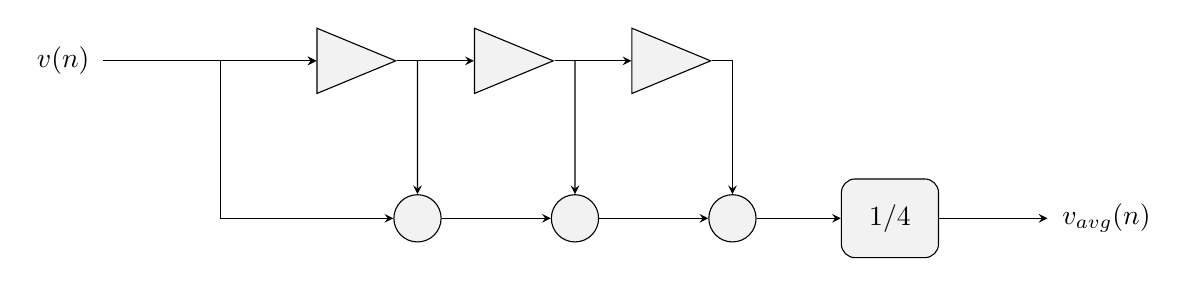
\begin{tikzpicture}[node distance = 2cm , >=stealth]
		% Place nodes
		\node [delay] (d1) {};
		\node [left of = d1, xshift=-1.5cm] (in) {$v(n)$};
		\node [delay, right of = d1] (d2) {};
		\node [delay, right of = d2] (d3) {};
		
		\draw [->] (d1)++(-1.5,0) to (d1);
		\draw [->] (d1) to (d2);
		\draw [->] (d2) to (d3);
		
		\node[sum, below of = d1, xshift=1cm] (s1) {};
		\node[sum, below of = d2, xshift=1cm] (s2) {};
		\node[sum, below of = d3, xshift=1cm] (s3) {};
		
		\draw [->] (d1)++(-1.5,0) |- (s1);
		\draw [->] (d2)++(-1,0) to (s1);
		
		\draw [->] (s1) to (s2);
		\draw [->] (d3)++(-1,0) to (s2);
		
		\draw [->] (s2) to (s3);
		\draw [->] (d3) -| (s3);
		
		\node [block, right of = s3] (fac) {1/4};
		\node [right of = fac, xshift=0.75cm] {$v_{avg}(n)$};
		
		\draw [->] (s3) to (fac);
		\draw [->] (fac) to ++(2,0);
		\draw [->] (d1)++(-3,0) to (d1);

	\end{tikzpicture} \end{center}

	\vspace{3em}
	
	The block diagram for (2):
	
	\begin{center} 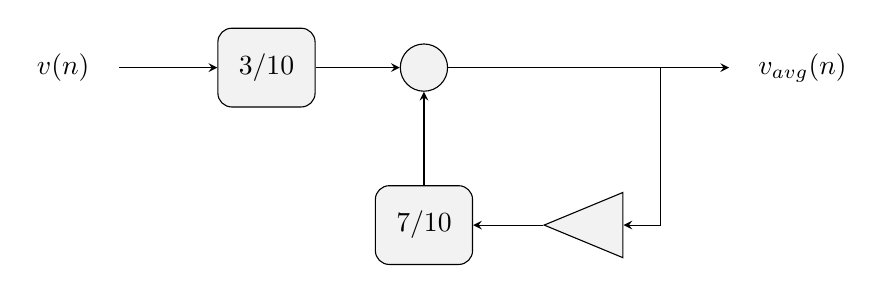
\begin{tikzpicture}[node distance=2cm, >=stealth]
		\node [label=left:$v(n)$] (in) {};	
		\node [block, right of = in] (fac1) {3/10};
		\node [sum, right of = fac1] (s1) {};
		\node [label=right:$v_{avg}(n)$, right of = s1, node distance=4cm] (out) {};
		\node [delay180, below of = s1, xshift=2.25cm] (d1) {};
		\node [block, below of = s1] (fac2) {7/10};
		
		\draw [->] (in) to (fac1);
		\draw [->] (fac1) to (s1);
		\draw [->] (s1) to (out);
		\draw [->] (out)++(-1,0) |- (d1);
		\draw [->] (d1) to (fac2);
		\draw [->] (fac2) to (s1);
	\end{tikzpicture}\end{center}
	
	\vspace{3em}
	
	The block diagram for (3):
	
	\begin{center} 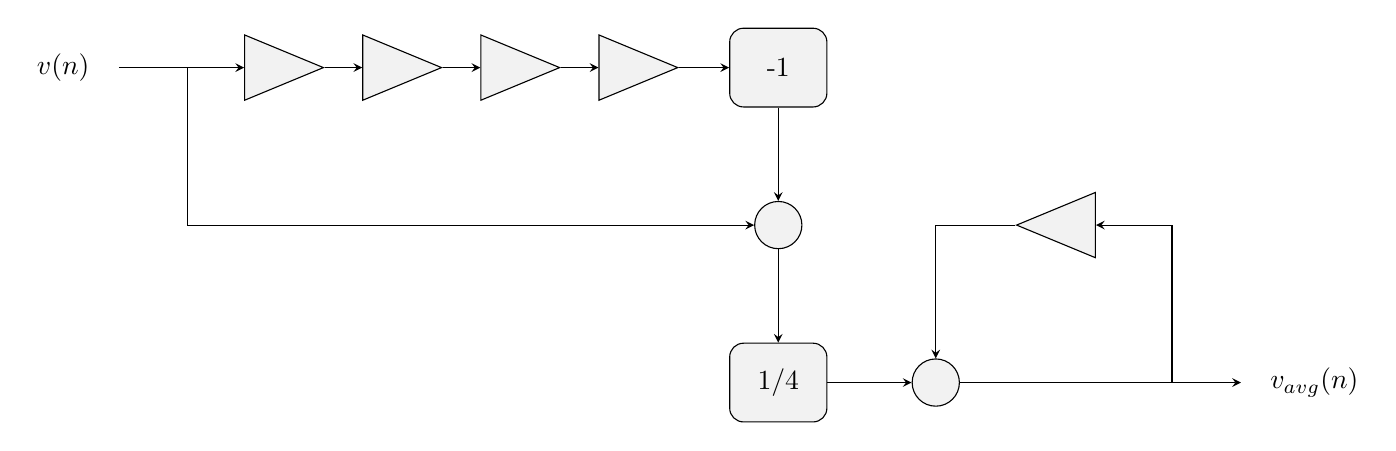
\begin{tikzpicture}[node distance=2cm, >=stealth]
		
		\node [label=left:$v(n)$] (in) {};
		\node [delay, right of = in] (d1) {};
		\node [delay, right of = d1, node distance=1.5cm] (d2) {};
		\node [delay, right of = d2, node distance=1.5cm] (d3) {};
		\node [delay, right of = d3, node distance=1.5cm] (d4) {};
		\node [block, right of = d4, node distance=2cm] (fac1) {-1};
		\node [sum, below of = fac1] (s1) {};
		\node [block, below of = s1] (fac2) {1/4};
		\node [sum, right of = fac2] (s2) {};
		\node [label=right:$v_{avg}(n)$, right of = s2, node distance=4cm] (out) {};
		\node [delay180, right of = s2, yshift = 2cm, xshift=-0.25cm] (d5) {};
		
		\draw [->] (in) to (d1);
		\draw [->] (d1) to (d2);
		\draw [->] (d2) to (d3);
		\draw [->] (d3) to (d4);
		\draw [->] (d4) to (fac1);
		\draw [->] (fac1) to (s1);
		\draw [->] (in)++(1,0) |- (s1);
		\draw [->] (s1) to (fac2);
		\draw [->] (fac2) to (s2);
		\draw [->] (s2) to (out);
		\draw [->] (out)++(-1,0) |- (d5);
		\draw [->] (d5) -| (s2);
	\end{tikzpicture}\end{center}

\section*{Impulse Response}

	To calculate impulse response, the following \texttt{MATLAB} script was created. 
	\vspace{1em}
	\begin{center}
		\includegraphics[scale=0.65]{Impulse Response Code.png}
	\end{center}
	\vspace{1em}
	This code provides the impulse response of (1), (2), and (3) plotted in red, green, and blue respectively. Additionally, the unit impulse was also plotted in black. 
	
	\textit{Note:} The red plot of (1) and blue plot of (3) overlap completely, thus the figure only shows the blue as it was plotted last.
	\vspace{1em}
	\begin{center}
		\includegraphics[scale=0.3]{Impulse Responses.png}
	\end{center}
	\vspace{1em}

\section*{Comparison of Algorithms}

	Lets start by analytically finding the impulse responses of (1) and (3), To find the impulse response, we can essentially treat $v(n) = \delta(n)$, where $\delta(n)$ is the dirac delta function. Performing this substitution we get (4) and (5) for the impulse responses of (1) and (3) respectively $\ldots$
	
	\begin{equation}
		v_{avg}(n) = \frac{1}{4} \left[ \delta(n) + \delta(n-1) + \delta(n-2) + \delta(n-3)  \right]
	\end{equation}
	
	\begin{equation}
		v_{avg}(n) = \frac{1}{4} \left[  \delta(n) - \delta(n-4) \right] + v_{avg}(n-1)
	\end{equation}
	
	The impulse response of (1), shown in (4), suggests that the dirac delta function is essentially \textit{spread out} over 4 time units, this means that essentially the dirac delta will appear in one out of every four terms for 4 time periods, this leads to the step of 0.25 seen on the impulse response.
	
	The impulse response of (3), shown in (5), suggests that the impulse response would be different due to the formula being different, however if we unbox the recursion we can start to see the similarities. Lets assume that the impulse appears at $t=0$, as well as 0 initial conditions.
	
	\begin{align*}
		v_{avg}(0) &= \frac{1}{4} (1 - 0) + 0 &= 0.25 \\
		v_{avg}(1) &= \frac{1}{4} (0 - 0) + v_{avg}(0) &= 0.25 \\
		v_{avg}(2) &= \frac{1}{4} (0 - 0) + v_{avg}(1) &= 0.25 \\
		v_{avg}(3) &= \frac{1}{4} (0 - 0) + v_{avg}(2) &= 0.25 \\
		v_{avg}(4) &= \frac{1}{4} (0 - 1) + v_{avg}(3) &= 0.00
	\end{align*}
	
	After unboxing the recursion, we can see that given 0 initial conditions, both (1) and (3) display the exact same finite impulse response. This essentially means that they process the signal the same way. (1) is a simple moving average filter, and (3) is some sort of (subtractive?) average with a recursion/feedback term that behaves the same. This similarity in processing can be seen in the included plot in the next section.

\section*{Data Processing}

	In order to process the data according to (1), (2), and (3), the following \texttt{MATLAB} script was developed
	\vspace{1em}
	\begin{center}
		\includegraphics[scale=0.65]{SPTSX Code.png}
	\end{center}
	This script outputs a plot of the original data in black, and the processed data with algorithms (1), (2), and (3) plotted in red, green, and blue respectively.
	\vspace{1em}
	\begin{center}
		\includegraphics[scale=0.3]{SPTSX.png}
	\end{center}
	\vspace{1em}
	From a quick look at the graph, we can easily see that the green trace seems to be smoother than the other extremely sharp traces, thus I think that the algorithm in (2) worked the best at smoothing out the data. I have provided a more zoomed in picture contrasting both plots on the next page, to help you see how much smoother the green trace is than the other ones. I think this makes sense because when an impulse (daily fluctuation) appears in (2) its impulse response suggests a smoothed out (diminishing) response which is smoother than the step on and off from (1) and (3).
	
	\textit{Note:} In the below images the blue trace has been shifted up by 12650 y-units to appear alongside the other traces. Also note the equivalency in fluctuations of the red and blue traces.
	
	\newpage
	
	\begin{center}
		\includegraphics[scale=0.3]{comparison1}
		\includegraphics[scale=0.3]{comparison2}
	\end{center}
	
\end{document}
